\documentclass[10pt,a4paper,twocolumn]{article}

\usepackage[
  a4paper,
  left=25mm,
  right=25mm,
  top=25mm,
  bottom=25mm,
  columnsep=6mm
]{geometry}

\usepackage[T1]{fontenc}
\usepackage[utf8]{inputenc}
\usepackage{mathpazo}             % Palatino text + math
\usepackage{microtype}            % Improved typographic quality
\linespread{1.0}                  % Single line spacing

% ── Essential packages ───────────────────────────────────────────────────
\usepackage{amsmath,amssymb}      % Mathematics
\usepackage{graphicx}             % Images
\usepackage{booktabs}             % Professional tables (\toprule, \midrule, \bottomrule)
\usepackage{caption}              % Caption formatting
\usepackage{float}                % Improved float placement
\usepackage{enumitem}             % List customization
\usepackage{url}                  % URL formatting
\usepackage{xcolor}               % Colours
\usepackage{fancyhdr}             % Headers and footers
\usepackage{titlesec}             % Section heading formatting
\usepackage{natbib}               % APA-style citations
\usepackage{tikz}
\usetikzlibrary{positioning,arrows.meta}
\usepackage{hyperref}             % Clickable links (load last)

% ── Colour definitions (BUas palette) ────────────────────────────────────
\definecolor{buasnavy}{HTML}{0F2A44}
\definecolor{buasteal}{HTML}{0D7377}
\definecolor{guidegray}{HTML}{5D6D7E}

\hypersetup{
  colorlinks=true,
  linkcolor=buasnavy,
  citecolor=buasteal,
  urlcolor=buasteal,
  pdfauthor={Vladislav Stoimenov},
  pdftitle={Road Damage Detection and Risk-Aware Geospatial Routing for Road Maintenance Prioritisation},
}

\captionsetup{
  font={bf,small},
  labelsep=colon,
  skip=6pt,
}
\captionsetup[table]{position=above}
\captionsetup[figure]{position=below, justification=centering}

\setlength{\tabcolsep}{4pt}

\titleformat{\section}
  {\normalfont\fontsize{12}{14}\bfseries}{\thesection}{1em}{}
\titlespacing*{\section}{0pt}{12pt}{3pt}

\titleformat{\subsection}
  {\normalfont\fontsize{10}{12}\bfseries}{\thesubsection}{1em}{}
\titlespacing*{\subsection}{0pt}{12pt}{3pt}

\titleformat{\subsubsection}
  {\normalfont\fontsize{10}{12}\itshape\bfseries}{\thesubsubsection}{1em}{}
\titlespacing*{\subsubsection}{0pt}{8pt}{2pt}

\pagestyle{fancy}
\fancyhf{}
\fancyfoot[R]{\small\thepage}
\renewcommand{\headrulewidth}{0pt}
\renewcommand{\footrulewidth}{0pt}

\setlength{\parindent}{6mm}
\setlength{\parskip}{0pt}

\begin{document}

\twocolumn[
  \begin{@twocolumnfalse}
  \begin{center}
    {\small\color{guidegray}
      Breda University of Applied Sciences \hspace{1em}$\mid$\hspace{1em}
      Academy of Games and Media \hspace{1em}$\mid$\hspace{1em}
      Data Science \& AI}
    \vspace{12pt}

    % ── Title ────────────────────────────────────────────────────────────
    % 16pt bold, small caps for lowercase letters. Content words begin
    % with a capital letter ('title caps'). Leave 3pt below the title.
    {\fontsize{16}{19}\bfseries\scshape
      Road Damage Detection and Risk-Aware Geospatial Routing for Road
      Maintenance Prioritisation
    \par}
    \vspace{3pt}

    {\normalsize Bachelor's Thesis}
    \vspace{6pt}

    % ── Author information ───────────────────────────────────────────────
    % Name, student number, email. Remove the student number from the
    % final version you upload to the repository.
    {\normalsize
      Vladislav Stoimenov, 235030, 235030@buas.nl}
    \vspace{2pt}

    {\normalsize
      Supervisor: Karna Rewatkar}
    \vspace{12pt}

    \begin{minipage}{0.92\textwidth}
      \small
      \setlength{\parindent}{6mm}

      \textbf{Abstract:}
      Road surface damage raises driving risk and maintenance costs, yet
      manual inspection does not scale to municipal road networks. This
      thesis presents and evaluates an end-to-end pipeline that detects road
      damage in street photographs, converts detections into interpretable
      risk scores, and uses those scores for risk-aware routing and
      maintenance prioritisation. YOLOv8n and Faster R-CNN were trained under
      matched conditions on a class- and country-balanced subset of RDD2022.
      YOLOv8n achieved higher mAP50-95 (0.300 versus 0.186) and substantially
      faster inference (median 22\,ms versus 307\,ms per image). Both models
      dropped sharply on manually collected photographs from Sofia
      (mAP50-95 of 0.041 and 0.040 respectively), and fine-tuning on 131 local images raised
      YOLOv8n's F1 from 0.19 to 0.35. Against independently labelled Sofia
      images, the rule-based risk classifier reached 59.5\% accuracy (macro
      F1 0.58, below the 0.75 target); its errors traced to missed detections
      rather than mis-scored ones. In a neighbourhood with recorded hazards,
      risk-aware routes reduced hazard exposure by a median of 37\% (mean 46\%)
      compared with shortest paths, with 95\% of routes within a 10\% distance
      increase (Wilcoxon $p = 0.0017$). Generated segment risk correlated with
      manual ratings (Spearman's $\rho = 0.68$). A lightweight detector adapted
      with modest local data, combined with explainable risk scoring, can
      support municipal maintenance decisions, with detection recall and local
      data coverage as the main constraints.
    \end{minipage}

    \vspace{6pt}
  \end{center}

  \end{@twocolumnfalse}
]

% ════════════════════════════════════════════════════════════════════════════
%  SECTION 1: INTRODUCTION
% ════════════════════════════════════════════════════════════════════════════
\section{Introduction}
\label{sec:introduction}

\subsection{Context and problem}
\label{sec:context-problem}

Road surface damage such as potholes, longitudinal cracking, transverse
cracking, and alligator cracking degrades driving safety and comfort, and
represents a recurring cost for municipal road authorities. Damage that
is left unrepaired tends to worsen over time, so identifying it early and
prioritising repairs accordingly is central to cost-effective road
maintenance. The conventional approach, manual visual inspection by
trained personnel, does not scale well to an entire municipal road
network: it is labour-intensive, infrequent by necessity, and produces
assessments that are difficult to compare consistently across inspectors
or over time.

Computer vision offers a scalable alternative. Convolutional object
detectors can be trained to localise and classify road damage directly
from photographs, removing the dependency on continuous manual
inspection and enabling damage records to be produced automatically from
images collected by ordinary vehicles, phones, or dedicated inspection
rigs. A large body of work, reviewed in Section~\ref{sec:related-work},
has demonstrated that this is technically feasible for the detection
step in isolation.

Detection alone, however, does not constitute a decision-support system.
A list of bounding boxes and class labels does not, by itself, tell a
municipality which streets to repair first, nor does it change how a
route is planned through a network that already contains known hazards.
Turning detections into something actionable requires two further steps:
translating each detection into an interpretable measure of risk, and
propagating that risk into the geospatial systems, such as road networks
and routing algorithms, that municipalities and drivers already use. This
thesis treats detection, risk scoring, and risk-aware routing as one
connected pipeline rather than as three separate problems, on the
argument that the practical value of automated road-damage detection is
realised only once its output is connected to a decision such as ``repair
this segment first'' or ``avoid this street''.

\subsection{Research questions and hypotheses}
\label{sec:research-questions}

The central research question addressed in this thesis is:

\begin{quote}
\emph{How can computer vision-based road damage detection be integrated
with risk-based geospatial routing to improve route safety and support
road maintenance prioritisation?}
\end{quote}

This question is decomposed into four sub-questions, each associated
with one hypothesis that is tested empirically in
Section~\ref{sec:results}.

\textbf{Sub-question 1.} Which object detection model performs best,
based on evaluation metrics such as mean average precision (mAP),
precision, and recall, for detecting road damage in images?

\begin{quote}
\textbf{H1:} YOLOv8 will achieve detection accuracy (mAP) within 2 percentage points (mAP50-95) of
Faster R-CNN, while maintaining lower computational complexity. A 2\%
difference in mAP is considered an acceptable performance margin for
comparing models of broadly similar accuracy.
\end{quote}

\textbf{Sub-question 2.} How can detected road damage be translated into
meaningful road risk scores for routing and maintenance prioritisation?

\begin{quote}
\textbf{H2:} A rule-based risk scoring model based on damage type and
size will effectively differentiate road segments into low, medium, and
high-risk categories.
\end{quote}

\textbf{Sub-question 3.} How does incorporating road damage risk into
routing algorithms influence route selection compared to traditional
shortest-path routing?

\begin{quote}
\textbf{H3:} Risk-aware routing will reduce route hazard exposure
compared to shortest-path routing, while maintaining a reasonable
increase in total route distance.
\end{quote}

\textbf{Sub-question 4.} To what extent can the proposed system support
municipalities in identifying and prioritising road maintenance more
efficiently?

\begin{quote}
\textbf{H4:} The system will enable identification of high-risk road
segments, which can support maintenance prioritisation decisions based on
aggregated risk scores.
\end{quote}

\subsection{Approach overview}
\label{sec:approach-overview}

The detection stage of the pipeline is trained on RDD2022
\citep{arya2024rdd2022}, a multi-national road damage image dataset, using
two object detection architectures evaluated under matched conditions:
YOLOv8n \citep{jocher2023ultralytics}, a single-stage detector, and Faster
R-CNN with a ResNet50-FPN backbone \citep{ren2015fasterrcnn}, a two-stage
detector. Both architectures are trained on three dataset scales and, at
the final scale, on an explicitly class- and country-balanced subset of
RDD2022, so that the comparison in Section~\ref{sec:res-h1} isolates the
effect of architecture rather than an accidental difference in training
data. Detected damage is converted into a per-detection risk score using
a fixed, explainable rule based on damage class and detection confidence,
and combined into image- and road-segment-level risk using the same
combination rule at both levels. Road segments are identified using
OpenStreetMap data accessed via OSMnx \citep{boeing2017osmnx}, and
segment-level risk is used to bias a shortest-path routing algorithm away
from known hazards. Because a model trained only on an international
benchmark dataset is not guaranteed to generalise to a specific
deployment area, the pipeline additionally includes a domain-adaptation
stage: both detectors are fine-tuned on a small set of manually collected
photographs from a real pilot neighbourhood (Sveta Troitsa, Sofia,
Bulgaria), and the resulting system, from detection through to routing,
is evaluated against real, independently collected ground truth from that
same area. Figure~\ref{fig:pipeline} summarises the pipeline and the
hypothesis tested at each stage.

\begin{figure*}[t]
  \centering
  \scalebox{0.9}{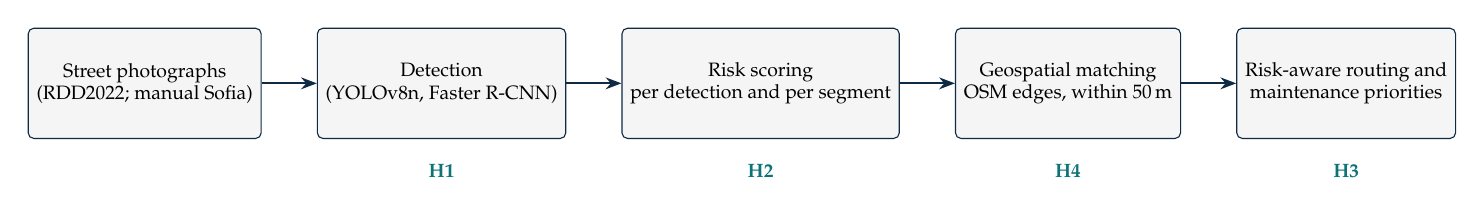
\begin{tikzpicture}[
    box/.style={draw=buasnavy, rounded corners=2pt, fill=gray!8,
      minimum width=25mm, minimum height=14mm, align=center,
      font=\scriptsize, inner sep=3pt},
    arr/.style={-{Stealth[length=2mm]}, draw=buasnavy, thick},
    tag/.style={font=\scriptsize\bfseries, text=buasteal}
  ]
    \node[box] (in) {Street photographs\\(RDD2022; manual Sofia)};
    \node[box, right=7mm of in] (det) {Detection\\(YOLOv8n, Faster R-CNN)};
    \node[box, right=7mm of det] (risk) {Risk scoring\\per detection and per segment};
    \node[box, right=7mm of risk] (geo) {Geospatial matching\\OSM edges, within 50\,m};
    \node[box, right=7mm of geo] (out) {Risk-aware routing and\\maintenance priorities};
    \draw[arr] (in) -- (det);
    \draw[arr] (det) -- (risk);
    \draw[arr] (risk) -- (geo);
    \draw[arr] (geo) -- (out);
    \node[tag, below=2mm of det] {H1};
    \node[tag, below=2mm of risk] {H2};
    \node[tag, below=2mm of geo] {H4};
    \node[tag, below=2mm of out] {H3};
  \end{tikzpicture}}
  \caption{Pipeline overview. Detections are converted into risk scores,
  matched to OpenStreetMap road segments, and used for risk-aware routing
  and maintenance prioritisation. H1--H4 mark the hypothesis tested at
  each stage.}
  \label{fig:pipeline}
\end{figure*}

\subsection{Contribution}
\label{sec:contribution}

This thesis makes three contributions. First, it provides a
model-comparison between YOLOv8n and Faster R-CNN that is repeated at
three dataset scales under matched training conditions, and tested with
formal statistical procedures (a paired significance test and a bootstrap
confidence interval, rather than a single point estimate) rather than
being asserted from one training run. Second, it quantifies the
generalisation gap between a detector trained purely on an international
benchmark and its performance on real, previously unseen photographs from
an actual deployment area, and measures how much of that gap a small,
low-cost domain-adaptation step can close. Third, it tests all four
hypotheses above against real, independently collected ground truth
rather than treating any of them as self-evidently true: a manually
labelled risk-classification sample for H2, a systematically generated
route sample for H3, and manually rated road segments for H4, each
analysed with an appropriate statistical test.


% ════════════════════════════════════════════════════════════════════════════
%  SECTION 2: RELATED WORK
% ════════════════════════════════════════════════════════════════════════════
\section{Related Work}
\label{sec:related-work}

\subsection{Road damage detection with computer vision}
\label{sec:rw-damage-detection}

Automated road damage detection has moved from small, single-country
image collections toward large, multi-national benchmarks. RDD2022
\citep{arya2024rdd2022} is one such benchmark, aggregating road images
from seven countries (Japan, India, the Czech Republic, Norway, the
United States, and two Chinese collection methods) and standardising
damage annotation around a small set of classes: longitudinal cracking,
transverse cracking, alligator cracking, and potholes, the same four
classes used throughout this thesis. Prior work built on this and
comparable benchmarks has repeatedly demonstrated that convolutional
object detectors, and single-shot detectors of the YOLO family in
particular \citep{redmon2016yolo,jocher2023ultralytics}, can localise and
classify these damage types with useful accuracy directly from
photographs. The Crowdsensing-based Road Damage Detection Challenge
\citep{arya2022crddc}, run on this same dataset, reported ensemble
submissions reaching an F1 score of around 0.76 on the held-out
challenge test set, giving a concrete, independently verified benchmark
figure against which the detector accuracies obtained in this thesis
(Section~\ref{sec:res-h1}) can be contextualised, bearing in mind that
the CRDDC figure comes from multi-model ensembles rather than the single
architectures compared here. This thesis reuses RDD2022 directly as its
primary training source (Section~\ref{sec:method-dataset}), rather than
proposing a new dataset, and instead focuses on a rigorous comparison of
detector architectures and on what happens once such a detector is
deployed on real, previously unseen images from one specific city.

\subsection{One-stage vs. two-stage detectors}
\label{sec:rw-detector-architectures}

Object detectors are broadly divided into two-stage detectors, which
first propose candidate regions and then classify and refine each one,
and one-stage (single-shot) detectors, which predict boxes and classes
directly over a dense grid in a single forward pass. Faster R-CNN
\citep{ren2015fasterrcnn} is the canonical two-stage architecture,
combining a region proposal network with a downstream classification and
bounding-box regression head; the YOLO family
\citep{redmon2016yolo,jocher2023ultralytics} is the canonical one-stage
alternative. The conventional framing in the literature is a speed-versus-accuracy
trade-off: two-stage detectors are often reported as more accurate,
particularly on small or densely packed objects, while one-stage
detectors are substantially faster and better suited to real-time or
resource-constrained deployment. H1 (Section~\ref{sec:research-questions})
is a direct operationalisation of this framing for the road-damage task,
predicting that YOLOv8 would trade a small amount of accuracy for a large
gain in computational efficiency. Whether the accuracy side of that
trade-off holds at the dataset scale used in this thesis is tested
directly in Section~\ref{sec:res-h1}, and is discussed in relation to
this framing in Section~\ref{sec:disc-h1}.

\subsection{Risk scoring and severity estimation for infrastructure}
\label{sec:rw-risk-scoring}

Pavement condition assessment has a long-established manual tradition,
typified by indices such as the Pavement Condition Index, which combine
observed distress type, severity, and extent into a single numerical
condition score used for maintenance planning \citep{shahin2005pci}.
The risk-scoring model used in
this thesis (Section~\ref{sec:method-risk-scoring}) follows the same
underlying logic, combining a fixed per-class severity weight with
detection confidence into a single interpretable score, but is
deliberately rule-based rather than learned, so that every score can be
traced back to an explainable cause. This is a deliberate simplicity
choice: a rule-based score is auditable by a non-technical stakeholder,
such as a municipal maintenance planner, in a way that a learned scoring
function is not.

\subsection{Geospatial routing with cost-augmented graphs}
\label{sec:rw-routing}

Routing algorithms that penalise undesirable segments by adding a cost
term to an otherwise standard shortest-path formulation are a
long-standing approach in navigation and logistics research, used, for
example, to route vehicles away from congestion, tolls, or known hazards
rather than purely minimising distance or travel time. A directly
analogous application outside the road-damage domain is
\citet{purchase2026saferoute}, who augment an OpenStreetMap-derived
street network with a crime-risk cost term to compute safer, rather
than strictly shortest, routes through a South African city, finding
that the risk-weighted route was on average substantially longer than
the shortest path but exposed travellers to roughly half the risk,
a trade-off pattern this thesis's own H3 result
(Section~\ref{sec:res-h3}) closely mirrors for road-damage risk rather
than crime risk. This thesis applies the same idea to
road damage risk: OpenStreetMap road network data, accessed through
OSMnx \citep{boeing2017osmnx}, is augmented with a risk-based cost term
per edge (Section~\ref{sec:method-routing}), and a standard shortest-path
algorithm is then run on the augmented graph exactly as it would be on
the unmodified one. The novelty in this thesis is not the routing
algorithm itself, which is deliberately kept simple and explainable, but
the fact that the cost term is derived from real, automatically detected
road damage rather than from static, pre-existing metadata such as road
class or speed limit.

\subsection{The gap this thesis fills}
\label{sec:rw-gap}

The great majority of road-damage detection literature stops at
detection metrics: precision, recall, and mAP on a held-out test split of
the same benchmark used for training. Comparatively little published work
connects detection output to a downstream decision, such as a
maintenance priority ranking or a routing decision, and fewer still
evaluate that downstream decision against independently collected,
real-world ground truth rather than against the same benchmark's own
labels. This thesis addresses that gap directly: every stage of the
pipeline, from detection through risk scoring to routing, is evaluated
against explicit, pre-registered hypotheses (H1--H4), and three of the
four hypotheses are tested against ground truth that was collected
independently of, and after, model training, rather than against a
held-out split of the same training distribution.


% ════════════════════════════════════════════════════════════════════════════
%  SECTION 3: METHODOLOGY
% ════════════════════════════════════════════════════════════════════════════
\section{Methodology}
\label{sec:methods}

\subsection{Dataset construction}
\label{sec:method-dataset}

All models are trained on subsets of RDD2022 \citep{arya2024rdd2022},
which provides 26\,869 training, 5\,758 validation, and 5\,758 test
images across seven national/collection sources (Japan, Norway, India,
the United States, the Czech Republic, and two Chinese collection
methods, drone- and motorbike-mounted). Only the four damage classes used
throughout this thesis, longitudinal cracking (D00), transverse cracking
(D10), alligator cracking (D20), and potholes (D40), are retained; a
fifth, unofficial class present in the raw converted labels is filtered
out at processing time.

Three processed datasets were built at increasing scale, summarised in
Table~\ref{tab:dataset-iterations}: an initial small dataset used to
validate that the full pipeline, from raw data to trained model to
evaluation, worked end to end; a medium dataset used for a first
scaled-up retrain; and a final, large dataset used for all results
reported in Section~\ref{sec:results}. Progressing through these scales
was necessary because auditing the small and medium datasets revealed two
compounding biases inherited from RDD2022's raw class and country
distribution. First, class~D00 outnumbered classes~D20 and~D40 by a
factor of two to three in both smaller datasets, despite D20 and D40
being the two highest-severity classes in the risk-scoring model
(Section~\ref{sec:method-risk-scoring}). Second, Japan accounted for
approximately 46\% of both smaller processed datasets, against
approximately 28\% of the raw pool, while the Czech Republic was
represented by zero images in the small dataset's validation split.

\begin{table}[t]
  \centering
  \small
  \caption{Dataset-size iterations used in this thesis. All splits are
  drawn from RDD2022's own train/val/test partitions, filtered to the
  four damage classes used in this thesis.}
  \label{tab:dataset-iterations}
  \begin{tabular}{lrrr}
    \toprule
    Dataset & Train & Val & Test \\
    \midrule
    Small  & 277   & 60  & 60  \\
    Medium & 1\,034 & 224 & 221 \\
    Large  & 4\,291 & 597 & 592 \\
    \bottomrule
  \end{tabular}
\end{table}

The large dataset was constructed with an explicit balancing procedure
rather than by simple random sampling. For each of the four classes, a
fixed per-class image quota (1\,100 training images, 150 validation, 150
test) was distributed as evenly as possible across every national source
that contains at least one example of that class, using a water-filling
allocation: countries are given an equal share of the quota, and any
shortfall from a country with too few available images is redistributed
across the remaining countries. This was necessary rather than optional,
because auditing raw class-by-country availability found that class~D40
has zero images from Norway, the United States, or the Czech Republic in
RDD2022 at all; a fixed seven-way split would have been infeasible for
this class, so the allocation is computed per class over only the
countries that actually contain it. A fixed number of damage-free
(``negative'') images (200 training, 30 validation) was additionally
included per split, so that the trained models also see undamaged road
surface as background.

\subsection{Model architectures and training configuration}
\label{sec:method-models}

The two architectures were chosen to represent the two detector families
compared in H1. YOLOv8n is the smallest variant of the current YOLO family
and is designed for fast inference on modest hardware, which matches the
deployment setting discussed in Section~\ref{sec:disc-implications}. Faster
R-CNN is the canonical two-stage detector and a long-established reference
point in object detection, providing a well-understood baseline for the
two-stage side of the comparison. Both have COCO-pretrained weights, so the
same starting point and training protocol can be applied to each.

Two object detection architectures are trained and compared, directly
operationalising H1: YOLOv8n \citep{jocher2023ultralytics}, a
lightweight, single-stage detector (approximately 3.0 million
parameters), and Faster R-CNN with a ResNet50 backbone and a feature
pyramid network \citep{ren2015fasterrcnn}, a two-stage detector
(approximately 43.3 million parameters), initialised from COCO-pretrained
weights in both cases.

Both architectures are trained identically at every dataset scale, so
that any measured difference reflects the architecture rather than an
incidental difference in training conditions: the same image resolution
(640\,px), the same train/validation/test split, and the same effective
batch size are used for both models at a given dataset scale
(Table~\ref{tab:training-params}). Because Faster R-CNN's memory
footprint is substantially larger than YOLOv8n's at a given batch size,
its effective batch size is reached through gradient accumulation
(a small number of images per forward/backward pass, with gradients
summed over several steps before an optimiser update) rather than a
single large batch, together with automatic mixed-precision training;
both measures reduce peak GPU memory without changing the effective
batch size, which was necessary given training was carried out on a
single local GPU with 8\,GB of memory. Both architectures use early
stopping on validation loss (YOLOv8n) or a fixed patience on validation
loss (Faster R-CNN), rather than a fixed epoch budget, so that neither
model is arbitrarily under- or over-trained relative to the other.

\begin{table}[t]
  \centering
  \small
  \caption{Training configuration at the final (large) dataset scale, applied
  identically to both architectures unless noted.}
  \label{tab:training-params}
  \begin{tabular}{@{}p{3.1cm}p{3.3cm}@{}}
    \toprule
    Parameter & Value \\
    \midrule
    Image size & 640\,px \\
    Effective batch size & 16 \\
    Maximum epochs & 100 \\
    Early stopping patience & 20 epochs (val.\ loss) \\
    Optimiser & SGD \\
    Mixed precision & Enabled (Faster R-CNN) \\
    Gradient accumulation & 4 steps (Faster R-CNN) \\
    \bottomrule
  \end{tabular}
\end{table}

\subsection{Risk-scoring model}
\label{sec:method-risk-scoring}

Each accepted detection (confidence at or above the detector's
confidence threshold) is converted into a per-detection risk score as
the product of a fixed, class-dependent base severity and a mild
confidence multiplier:

\begin{equation}
  \label{eq:detection-risk}
  r_i = s_{c_i} \cdot m(p_i),
\end{equation}

where $r_i$ is the risk score of detection $i$, $c_i$ is its damage
class, $s_{c_i}$ is that class's fixed base severity
(Table~\ref{tab:severity}), and $p_i$ is its confidence. The confidence
multiplier is defined as

{\footnotesize
\begin{equation}
  \label{eq:confidence-multiplier}
  m(p) =
  \begin{cases}
    m_{\min} & p \leq \tau \\
    m_{\min} + \tfrac{p - \tau}{1 - \tau}(1 - m_{\min}) & \tau < p < 1 \\
    1 & p \geq 1,
  \end{cases}
\end{equation}
}

with confidence floor $m_{\min} = 0.7$ and confidence threshold
$\tau = 0.25$ (the same threshold at which a detection is accepted at
all). The multiplier is deliberately narrow, spanning only $[0.7, 1.0]$,
rather than the full $[0,1]$ range: a detection's confidence reflects how
sure the model is that the damage is present, not how physically
dangerous it is once confirmed, so a low-confidence real pothole should
not be scored as though it were only mildly hazardous.

\begin{table}[t]
  \centering
  \small
  \caption{Fixed base severity per damage class.}
  \label{tab:severity}
  \begin{tabular}{lr}
    \toprule
    Class & Base severity $s_c$ \\
    \midrule
    D00 -- Longitudinal crack & 1.0 \\
    D10 -- Transverse crack   & 1.2 \\
    D20 -- Alligator crack    & 2.0 \\
    D40 -- Pothole            & 3.0 \\
    \bottomrule
  \end{tabular}
\end{table}

Bounding-box size is deliberately excluded from the severity
calculation, which is a departure from the original proposal wording of
H2 (``damage type \emph{and size}''). In a single two-dimensional
photograph, the apparent size of a bounding box is a function of camera
distance and angle at least as much as it is a function of the real-world
size of the damage; using it as a severity multiplier would let camera
technique, rather than the underlying road condition, distort the risk
score. This deviation is stated explicitly here, and its consequences for
H2 are discussed in Section~\ref{sec:disc-h2}.

Multiple detections, whether within a single photograph or matched to
the same road segment, are combined with the same rule at both levels:

\begin{equation}
  \label{eq:combine}
  R = \max_i(r_i) + \beta \sum_{j \neq \arg\max_i(r_i)} r_j,
\end{equation}

with damping factor $\beta = 0.3$. The single worst detection dominates
the combined score, so that one severe hazard is not diluted by several
minor ones, while additional co-occurring damage still increases the
score rather than being ignored. At image level, the combined score $R$
is normalised to $[0,1]$ by dividing by a ceiling equal to the highest
base severity (3.0, so that one confidently detected pothole alone
already saturates the score), and categorised as low
($<0.34$), medium ($0.34$--$0.67$), or high ($\geq 0.67$).

A combined risk score should satisfy three criteria: (i) the single worst
hazard should dominate the score; (ii) additional damage should still
increase the score; and (iii) confidence should only nudge the score within
a narrow range, rather than deciding it. To illustrate how alternative
combination rules meet these criteria, consider the photograph Test\_Route\_16 (Figure~\ref{fig:test-route-16}),
processed by the deployed pipeline. It contains five accepted detections: one transverse crack (D10, confidence
0.587, per-detection risk 1.002) and four longitudinal cracks (D00, with
confidences 0.754, 0.427, 0.402 and 0.372, and per-detection risks 0.902,
0.771, 0.761 and 0.749). Four scoring rules applied to these detections give
the following results on the 0--1 scale:

\begin{itemize}
  \item \textbf{Severity only} (highest base severity present, 1.2):
  $1.2 / 3.0 = 0.40$, medium. The four longitudinal cracks and all
  confidence information are ignored.
  \item \textbf{Sum of base severities, no confidence}: $5.2 / 3.0$
  saturates at 1.0, high. Five modest cracks dominate the score.
  \item \textbf{Highest confidence only} (0.754): 0.75, high. The class of
  each detection, and the other four detections, are ignored.
  \item \textbf{Current rule} (Equations~\ref{eq:detection-risk}--\ref{eq:combine}):
  $1.002 + 0.3 \times 3.183 = 1.957$, normalised to 0.652, medium.
\end{itemize}

Against these criteria, severity-only fails (ii) and (iii): the four
longitudinal cracks have no effect on the score, and confidence has no
effect at all. Summing severities fails (i), since five modest cracks
outweigh the worst one, and fails (iii), since confidence is ignored.
Highest confidence only fails (i), since the most severe damage does not
decide the score, and fails (iii), since confidence decides the whole score
rather than nudging it. The current rule meets all three: the transverse
crack contributes 1.002 of the 1.957 total (51\%), the four cracks together
add 0.955, and confidence moves each longitudinal crack only within the
multiplier range $[0.7, 1.0]$ (0.749 at confidence 0.372, 0.902 at 0.754).
The example illustrates how each rule behaves against these criteria; it is
not evidence that the current rule is more accurate than the alternatives,
since H2 is not supported at its target threshold
(Section~\ref{sec:res-h2}). The resulting score of 0.652 also lies close to
the medium/high boundary of 0.67, so a small change in the rule would
change this category.

\begin{figure}[t]
  \centering
  \includegraphics[width=\columnwidth]{figures/test_route_16_detections}
  \caption{Test\_Route\_16 with the five accepted detections used in the
  worked example. Red boxes show the detector's output; each label gives the
  damage type and confidence.}
  \label{fig:test-route-16}
\end{figure}

\subsection{Geospatial matching and risk-aware routing}
\label{sec:method-routing}

The routing and geospatial-matching components of the pipeline are
scoped to a single real pilot area, Sofia, Bulgaria, rather than the
whole of Bulgaria, on the grounds that the intended use case is a
municipal tool and a city-scale road network is both sufficient to
demonstrate the pipeline and small enough to download and route over
efficiently. The Sofia drivable road network (an 8\,km radius around the
city centre, 11\,363 nodes and 27\,429 edges) is obtained from
OpenStreetMap via OSMnx \citep{boeing2017osmnx} and cached locally.

Each detection's GPS coordinate is matched to the nearest edge in this
graph, identified by its two endpoint node identifiers and a key
disambiguating parallel edges between the same two nodes. A match is
accepted only if the nearest edge is within a fixed distance threshold
(50\,m); points further away, or outside the graph's bounding box
entirely, are left unmatched rather than force-matched to a plausible but
potentially incorrect road. All detections matched to the same edge are
combined into a segment-level risk using Equation~\ref{eq:combine}
applied over that edge's detections, producing two figures: an
unnormalised \emph{total risk}, used for maintenance-priority ranking,
and a \emph{risk density}, the total risk divided by the segment's
real-world length, used for routing, so that a long segment is not
penalised more heavily purely for having had more opportunities to be
photographed.

The risk-aware routing algorithm adds a risk-based cost term to each
edge's physical length:

\begin{equation}
  \label{eq:routing-cost}
  c(e) = \ell(e) + \alpha \cdot d(e),
\end{equation}

where $c(e)$ is the edge's routing cost, $\ell(e)$ its length in metres,
$d(e)$ its risk density (zero for edges with no matched detections), and
$\alpha$ a weighting constant. A standard shortest-path algorithm is then
run twice on the same graph: once using $\ell(e)$ alone (the
``shortest'' route), and once using $c(e)$ (the ``risk-aware'' route).
The value $\alpha = 15\,000$ was set empirically against the available
pilot data: below this value, the extra distance cost of detouring
around the single highest-risk known segment outweighed its risk penalty
and the shortest and risk-aware routes coincided; at this value, avoiding
that segment became worthwhile. This is a rule-based prototype value
rather than a calibrated safety threshold, and is exposed as an
adjustable parameter in the deployed application rather than fixed in
code.

\subsection{Prototype implementation}
\label{sec:method-prototype}

The deployed system is a web prototype built with Streamlit (version
1.62), with interactive maps rendered using Folium. It consists of four
pages that follow the order of the pipeline. Screenshots of each page are
provided in Appendix~\ref{app:app-screenshots}.

\begin{itemize}
  \item \textbf{Dashboard} summarises all stored observations: the number
  of processed images, detected damages, affected road segments, the
  average risk score, and the number of high-risk locations, together with
  detections per damage class, observations per risk category, and an
  overview map.
  \item \textbf{Upload and Detect} accepts a geotagged street photograph,
  runs the detector, and displays the annotated image, each accepted
  detection with its confidence and risk contribution, and the observation
  risk. An observation is stored only when the user confirms it. Each
  file is identified by a SHA-256 hash of its contents, so re-uploading an
  identical image is recognised.
  \item \textbf{Damage Map} shows every stored observation as a marker and
  the road segments with recorded damage, coloured by segment risk, with an
  optional risk heatmap layer.
  \item \textbf{Safer Route Planner} takes an origin and a destination on
  the road network, computes the shortest and the risk-aware route, and
  reports their distance and hazard exposure. The risk-aversion weight
  $\alpha$ (Equation~\ref{eq:routing-cost}) is adjustable on this page.
\end{itemize}

Detection, risk scoring, routing, and storage run locally. All records are
held in a single SQLite database file, and uploaded images are kept in a
local upload folder. The database has four tables, summarised in
Table~\ref{tab:db-schema}, and the road network is loaded from the cached
OpenStreetMap graph described in Section~\ref{sec:method-routing}. The only
external data loaded by the application is the map tile imagery.

\begin{table}[t]
  \centering
  \small
  \caption{Tables in the local SQLite database.}
  \label{tab:db-schema}
  \begin{tabular}{@{}p{2.1cm}p{5.1cm}@{}}
    \toprule
    Table & Stored content (one row per) \\
    \midrule
    \texttt{observations} & saved image: file hash (unique, so duplicate uploads are rejected), GPS coordinate and its source (EXIF, manual, or map selection), upload time, model version, confidence threshold, inference time, observation risk score and category, and matched road edge with matching distance \\
    \texttt{detections} & accepted detection: damage class, confidence, bounding box, and risk contribution \\
    \texttt{road\_segments} & matched road edge: aggregated risk, risk density, risk category, and number of observations \\
    \texttt{routes} & route comparison: origin, destination, $\alpha$ used, shortest and risk-aware distance and exposure, and distance increase \\
    \bottomrule
  \end{tabular}
\end{table}

Recording the model version, confidence threshold, and matched road edge
with each observation allows any displayed result to be traced back to the
configuration that produced it. The 10\% distance limit used in H3 is
applied in the offline analysis: the application records the distance
increase of each route but does not enforce the limit.

Figure~\ref{fig:workflow} shows the workflow from the user's perspective,
with one lane for each group of actors.

\begin{figure*}[t]
  \centering
  \includegraphics[width=\textwidth]{figures/user_perspective_workflow}
  \caption{User-perspective workflow. A data collector uploads a geotagged
  photograph; the system detects damage, scores it, and stores the
  observation after the user confirms it. Municipal staff use the Damage Map
  to rank road segments, and drivers pick an origin and destination to compare
  routes. The first two lanes describe the implemented application, with
  recording done on a phone outside it; the bottom lane describes intended
  use.}
  \label{fig:workflow}
\end{figure*}

\subsection{Manual data collection and annotation}
\label{sec:method-manual-collection}

Two separate sets of manually collected road photographs were used in
this thesis, for two different purposes.

The first set comprises 201 road-damage photographs, independently
collected and manually annotated by the author for the four damage
classes used throughout this thesis. Images were obtained by mounting a
smartphone camera inside the car and recording continuous video while
driving on public roads around Sofia, outside the Sveta Troitsa area
subsequently used for the routing and heatmap-validation evaluations
(Sections~\ref{sec:res-h3} and~\ref{sec:res-h4}), so that the images used
for fine-tuning and the images used for those two evaluations do not
overlap. Individual frames containing visible damage were then extracted
from the recorded video and annotated using CVAT (Computer Vision
Annotation Tool), exported in the Ultralytics YOLO Detection~1.0 format
(normalised bounding boxes, class identifiers 0--3 matching the same
convention used for RDD2022). No single fixed camera angle was imposed:
because frames were sampled from continuous driving footage, the
resulting images naturally cover a range of distances and viewing angles
to the road surface, which was intentional, so that the fine-tuned
models would not be trained on an artificially narrow viewpoint and
would generalise better to images captured from different angles at
deployment time. Every image/label pair in this set was verified
programmatically before use: that every image has a corresponding label
file and vice versa, that every label file contains only valid class
identifiers and in-range normalised coordinates, and that the damage
class indicated in each file's name is actually present among its own
annotated classes; all 201 pairs passed these checks. The resulting class
distribution is imbalanced (150, 75, 90, and 35 images containing at
least one D00, D10, D20, and D40 instance respectively), which is
discussed as a limitation in Section~\ref{sec:disc-limitations}. None of
the 201 images retain GPS metadata, since frame extraction from video
does not preserve the per-frame location information a native photo
capture would. Because of this, the set was used for the
domain-adaptation fine-tuning and held-out evaluation described below,
which do not require location information, but not for the geospatial
matching and routing evaluation (Sections~\ref{sec:method-routing},
\ref{sec:res-h3} and~\ref{sec:res-h4}), which do.

Examples of annotated frames from this set are shown in
Figure~\ref{fig:dataset-examples}.

\begin{figure*}[t]
  \centering
  \includegraphics[width=0.75\textwidth]{figures/dataset_examples}
  \caption{Example annotations from the manually collected Sofia dataset
  for the four damage classes used in this thesis, with ground-truth
  bounding boxes in red. Images are shown for illustration only; they are
  drawn from the same set used for fine-tuning and held-out evaluation.}
  \label{fig:dataset-examples}
\end{figure*}

The second set comprises 17 photographs collected specifically to
support the routing and heatmap-validation evaluations
(Sections~\ref{sec:res-h3} and~\ref{sec:res-h4}), for which real
coordinates were required. These were taken with the same smartphone as
the first set, but not while driving: the device's standard camera
application was used to photograph individual sections of damage that were
judged worth recording within the neighbourhood, rather than extracting
frames from continuous video. Location services were enabled so that GPS coordinates were
retained in each image's EXIF metadata. Unlike the first set, this set
was deliberately restricted to within a single pilot neighbourhood,
Sveta Troitsa, Sofia, covering its main streets; the neighbourhood's
evaluation boundary was subsequently derived directly from the actual
GPS extent of these photographs, rather than being predefined. Unlike
the first set, these images were not manually annotated; they were
instead processed directly through the same detection and risk-scoring
pipeline used by the deployed application, so that the risk data they
contribute reflects the system's own detections rather than
human-labelled ground truth.

\subsection{Domain-adaptation fine-tuning}
\label{sec:method-finetuning}

A model trained exclusively on RDD2022 is not guaranteed to generalise to
a specific deployment area: RDD2022's images were collected under
capture protocols, camera hardware, and road/lighting conditions specific
to its seven source countries, none of which is Bulgaria. To test and
address this, 201 photographs were independently collected and manually
annotated in the pilot area (Sveta Troitsa, Sofia), verified for label
consistency, and split into three non-overlapping subsets
(Table~\ref{tab:sofia-split}): a fine-tuning training set, a small
fine-tuning validation set used to monitor for overfitting during
fine-tuning, and a held-out test set that neither model was trained or
fine-tuned on at any stage, used exclusively for the before/after
comparison in Section~\ref{sec:res-domain-adaptation}.

\begin{table}[t]
  \centering
  \small
  \caption{Manual Sofia dataset split used for domain adaptation.}
  \label{tab:sofia-split}
  \begin{tabular}{lr}
    \toprule
    Split & Images \\
    \midrule
    Fine-tuning train & 131 \\
    Fine-tuning validation & 28 \\
    Held-out test & 42 \\
    \bottomrule
  \end{tabular}
\end{table}

Both large-dataset-trained models were fine-tuned on the 131-image
fine-tuning split, starting from their RDD2022-large weights, using a
reduced learning rate relative to training from scratch and a short
epoch budget with aggressive early stopping. The intent is a targeted
adjustment of existing weights toward the pilot area's visual conditions,
not a retrain: 131 images is a small fraction of the 4\,291-image
RDD2022-large training set, and a reduced learning rate limits how far
the already-learned representations can move.

\subsection{Evaluation and statistical analysis plan}
\label{sec:method-evaluation}

Detection performance is reported using precision, recall, F1, mean
average precision at an IoU threshold of 0.5 (mAP50), and averaged over
IoU thresholds from 0.5 to 0.95 (mAP50-95), computed identically for both
architectures on the same test splits.

Each metric answers a different question. Precision is the fraction of
predicted damage that is correct, and recall is the fraction of real damage
that is detected. F1 combines the two into a single value, so that models
can be ranked on one number. Object detection also requires that a predicted
box overlaps the ground-truth box. Intersection over Union (IoU) measures
this overlap as the area of the intersection divided by the area of the
union, and a detection counts as correct when its IoU reaches a threshold.
mAP50 uses a threshold of 0.5, a lenient localisation criterion, while
mAP50-95 averages over thresholds from 0.5 to 0.95 and so rewards accurate
box placement. mAP is the standard summary metric for object detection. It is
reported alongside F1 because the RDD2022 challenge reports F1
\citep{arya2022crddc}, which allows the results to be compared with that
benchmark.

H1's two criteria are each tested with a statistical procedure suited to
the specific claim being made, rather than a single generic test. The
complexity criterion (lower training and inference cost) is tested with
a paired Wilcoxon signed-rank test on per-image inference time, measured
for both architectures on the same set of test images in the same
session; the Wilcoxon test is used, rather than a paired $t$-test,
because inference-time distributions are typically right-skewed rather
than normally distributed. The accuracy criterion (mAP50-95 within two
percentage points) is an equivalence claim, not a claim of zero
difference, so it is tested with a bootstrap confidence interval on the
mAP50-95 difference between the two architectures (300 resamples of the
test set, with replacement), following the logic of two one-sided
equivalence tests: H1's accuracy criterion is considered supported only
if this interval falls entirely within $\pm 2$ percentage points, rather
than by inspecting whether a single point-estimate difference happens to
be small.

H2 is tested by comparing the deployed pipeline's automatically
generated low/medium/high risk category against an independently
assigned ground-truth label for the same images, using accuracy,
per-category precision/recall/F1, and Cohen's $\kappa$; $\kappa$ is
reported alongside raw accuracy because, with three categories, a
nontrivial level of agreement is expected by chance alone, and $\kappa$
corrects for this. The pre-registered target for H2 is a macro-averaged
F1 of at least 0.75.

H3 is tested by generating a fixed number of independent
origin-destination pairs, comparing the shortest and risk-aware route for
each, and applying a paired Wilcoxon signed-rank test to the hazard
exposure of the two routes across the sample. Hazard exposure of a route is
the sum, over every road segment the route traverses, of that segment's total
risk (Equation~\ref{eq:combine}, applied to all detections matched to the
segment); segments without recorded risk contribute zero. Exposure reduction
is the percentage by which the risk-aware route's exposure falls below the
shortest route's. The measure reflects both how many damaged segments a route
passes and how severe they are, so avoiding one high-risk segment counts for
more than passing several minor ones. Because the routing cost and the exposure
measure are both computed from the same recorded risk, H3 shows that the
risk-aware route avoids recorded damage, not that it avoids all damage in the
area. The same non-parametric
justification applies as for the complexity criterion above, and is
additionally appropriate given that many routes are expected to have
identical exposure on both sides (no hazard on the shortest path at all).
The hypothesis asks for a ``reasonable'' increase in route distance; this
is operationalised as an increase of at most 10\% over the shortest route,
and a route satisfies the constraint if it meets this limit.

H4 is tested with Spearman's rank correlation coefficient between
independently assigned segment risk ratings and the pipeline's generated
segment-level risk. Spearman's $\rho$, rather than Pearson's $r$, is used
because the manual ratings are an ordinal scale with a small number of
distinct values, for which a rank-based correlation is the more
appropriate measure of monotonic association. H4 is supported if $\rho$ is
at least 0.5 and $p$ is below 0.05.

In every case, ground truth used for H2 and H4 was assigned by looking at
the image or road segment in question alone, before the model's output
was consulted, so that the comparison is not biased by anchoring the
manual judgement to the model's answer.

\subsection{Qualitative usability evaluation}
\label{sec:method-qualitative}

The hypothesis tests above are quantitative and evaluate the pipeline's
outputs against ground truth; they do not speak to how a human user
experiences or trusts the system, which is a separate and complementary
question. To address this, a small qualitative usability evaluation was
conducted, following the Research Quality Guidelines' allowance for
qualitative methods, such as structured feedback and content analysis, to
complement quantitative results.

Ten participants each completed the same short, guided walkthrough of the deployed application: uploading a
photograph and reviewing its detection result, exploring the Damage Map,
comparing a shortest route against a risk-aware route in the Safer Route
Planner, and explaining, unprompted, what the displayed risk score and
colour coding meant to them. Each participant then completed a short
survey consisting of five closed, five-point Likert-scale questions
covering ease of understanding, intuitiveness of the risk categories, map
clarity, trust in the system's risk assessment, and perceived usefulness
of the route comparison, followed by four open-ended questions on
confusion points, trust, desired improvements, and general comments. The
closed questions are analysed with descriptive statistics (mean, median);
the open-ended responses are analysed qualitatively by grouping them into
recurring themes, following standard content-analysis practice, with
representative quotations retained for illustration. This design was
chosen specifically because the trust and clarity questions map directly
onto H2 and H4: H2 tests whether the risk-scoring rule is quantitatively
accurate, while this survey tests whether users independently perceive
that same risk information as trustworthy and clear, a distinct but
related question that the quantitative hypothesis tests cannot answer on
their own.

% ════════════════════════════════════════════════════════════════════════════
%  SECTION 4: RESULTS
% ════════════════════════════════════════════════════════════════════════════
\section{Results}
\label{sec:results}

\subsection{Quantitative results}
\label{sec:res-quantitative}

Quantitative results were collected from four distinct evaluation
procedures, each matched to the hypothesis it tests
(Section~\ref{sec:method-evaluation}): automated detection metrics
(precision, recall, F1, mAP) computed on each dataset scale's own
RDD2022 test split and, separately, on the held-out Sofia test set
before and after fine-tuning; a paired statistical comparison of the two
architectures on shared test data; a manually labelled sample of 42
Sofia images for risk-classification agreement (H2); a systematically
generated sample of routing comparisons (H3); and a manually rated
sample of road segments correlated against generated segment risk (H4).
Each is reported in turn below. Table~\ref{tab:hyp-summary} summarises
the four hypothesis tests, and the criteria are defined in
Section~\ref{sec:method-evaluation}.

\begin{table}[t]
  \centering
  \small
  \caption{Summary of hypothesis tests.}
  \label{tab:hyp-summary}
  \begin{tabular}{@{}p{1.7cm}p{2.1cm}p{1.9cm}p{1.3cm}@{}}
    \toprule
    Hypothesis & Criterion & Result & Verdict \\
    \midrule
    H1 & mAP50-95 gap within $\pm$2\,pp; lower inference time & CI outside margin; time $p{=}6.04{\times}10^{-99}$ & Partially supported \\
    H2 & Macro F1 $\geq$ 0.75 & Macro F1 0.582 & Not supported \\
    H3 & Lower exposure; distance increase $\leq$ 10\% & $p{=}0.0017$; 38/40 within limit & Supported \\
    H4 & $\rho \geq 0.5$, $p < 0.05$ & $\rho{=}0.683$ ($p{=}0.0036$) & Supported \\
    \bottomrule
  \end{tabular}
\end{table}

\subsubsection{Detection performance across dataset iterations}
\label{sec:res-iterations}

Table~\ref{tab:iteration-results} reports detection performance for both
architectures at all three dataset scales, on each scale's own RDD2022
test split. Both architectures improve monotonically and substantially as
the dataset grows: YOLOv8n's mAP50-95 increases from 0.119 at the small
scale to 0.300 at the large scale, and Faster R-CNN's from 0.043 to
0.186. YOLOv8n outperforms Faster R-CNN at every scale on every reported metric
except precision at the medium scale, where Faster R-CNN is higher
(0.543 versus 0.503).

\begin{table*}[t]
  \centering
  \small
  \caption{Detection performance across dataset-size iterations, evaluated on
  each scale's own RDD2022 test split.}
  \label{tab:iteration-results}
  \begin{tabular}{llrrrrr}
    \toprule
    Model & Dataset & Precision & Recall & F1 & mAP50 & mAP50-95 \\
    \midrule
    YOLOv8n       & Small  & 0.368 & 0.305 & 0.334 & 0.297 & 0.119 \\
    YOLOv8n       & Medium & 0.503 & 0.434 & 0.466 & 0.424 & 0.194 \\
    YOLOv8n       & Large  & \textbf{0.643} & \textbf{0.496} & \textbf{0.560} & \textbf{0.548} & \textbf{0.300} \\
    Faster R-CNN  & Small  & 0.227 & 0.205 & 0.216 & 0.136 & 0.043 \\
    Faster R-CNN  & Medium & 0.543 & 0.300 & 0.387 & 0.340 & 0.148 \\
    Faster R-CNN  & Large  & 0.434 & 0.379 & 0.404 & 0.373 & 0.186 \\
    \bottomrule
  \end{tabular}
\end{table*}

At the large scale, per-class mAP50-95 (Table~\ref{tab:per-class}) shows
that D40 (pothole), the class targeted most directly by the class-balancing
procedure (Section~\ref{sec:method-dataset}) and the highest-severity class
in the risk-scoring model, is the strongest class for both architectures,
a reversal of the pattern observed before balancing was introduced.

\begin{table}[t]
  \centering
  \small
  \caption{Per-class mAP50-95 on the large-dataset RDD2022 test split.}
  \label{tab:per-class}
  \begin{tabular}{@{}lrr@{}}
    \toprule
    Class & YOLOv8n & Faster R-CNN \\
    \midrule
    D00 -- Longitudinal crack & 0.211 & 0.131 \\
    D10 -- Transverse crack   & 0.226 & 0.164 \\
    D20 -- Alligator crack    & 0.316 & 0.169 \\
    D40 -- Pothole            & \textbf{0.448} & \textbf{0.277} \\
    \bottomrule
  \end{tabular}
\end{table}

\subsubsection{Domain-adaptation results}
\label{sec:res-domain-adaptation}

Evaluated on the RDD2022 large-dataset test split, YOLOv8n and Faster
R-CNN reach mAP50-95 of 0.300 and 0.186 respectively
(Table~\ref{tab:iteration-results}). Evaluated instead on the held-out
Sofia test set, without any fine-tuning, both collapse to approximately
the same low level: 0.041 for YOLOv8n and 0.040 for Faster R-CNN, a
relative drop of approximately 86\% and 78\% respectively
(Table~\ref{tab:domain-gap}). Both architectures collapsing to
approximately the same absolute performance despite very different
RDD2022-native performance is consistent with a genuine domain-shift
effect rather than a weakness specific to one architecture.

\begin{table}[t]
  \centering
  \footnotesize
  \caption{mAP50-95 on the RDD2022 test set versus the held-out Sofia test
  set, before any fine-tuning.}
  \label{tab:domain-gap}
  \begin{tabular}{@{}lrr@{}}
    \toprule
    Model & RDD2022 & Sofia (no FT) \\
    \midrule
    YOLOv8n       & 0.300 & 0.041 \\
    Faster R-CNN  & 0.186 & 0.040 \\
    \bottomrule
  \end{tabular}
\end{table}

Fine-tuning both models on the 131-image fine-tuning split and
re-evaluating on the same held-out Sofia test set produces a substantial
improvement for both architectures (Table~\ref{tab:finetune-results}):
YOLOv8n's F1 improves from 0.189 to 0.347 (a relative increase of
approximately 83\%), and Faster R-CNN's from 0.218 to 0.311 (approximately
43\%). YOLOv8n's absolute mAP50-95 gain (+0.107) is approximately five
times Faster R-CNN's (+0.021). Neither model's fine-tuned Sofia
performance reaches its RDD2022-native performance. The fine-tuned
YOLOv8n achieves a recall of 0.335 on this held-out test set.

\begin{table}[t]
  \centering
  \small
  \caption{Held-out Sofia test set performance, before and after
  domain-adaptation fine-tuning.}
  \label{tab:finetune-results}
  \begin{tabular}{@{}llrr@{}}
    \toprule
    Model & Stage & F1 & mAP50-95 \\
    \midrule
    YOLOv8n      & No fine-tuning & 0.189 & 0.041 \\
    YOLOv8n      & Fine-tuned     & \textbf{0.347} & \textbf{0.148} \\
    Faster R-CNN & No fine-tuning & 0.218 & 0.040 \\
    Faster R-CNN & Fine-tuned     & 0.311 & 0.061 \\
    \bottomrule
  \end{tabular}
\end{table}

\subsubsection{H1 -- model comparison}
\label{sec:res-h1}

H1's two criteria were tested independently on the large-dataset models
(Table~\ref{tab:h1-verdict}). The accuracy criterion, that YOLOv8n's mAP50-95
would fall within two percentage points of Faster R-CNN's, is rejected: a
300-resample bootstrap over the shared test set gives a 95\% confidence
interval of $[+0.086, +0.117]$ on the YOLOv8n$-$Faster R-CNN mAP50-95
difference, entirely outside the $\pm 0.02$ equivalence margin. The
complexity criterion is supported: a paired Wilcoxon signed-rank test on
per-image inference time (median 22.25\,ms for YOLOv8n versus 307.33\,ms
for Faster R-CNN, measured on the same 592 test images in the same
session) gives $p = 6.04 \times 10^{-99}$. Training wall-clock time shows
the same pattern: 1.36\,hours for YOLOv8n (100 of 100 epochs, no early
stop) against 4.16\,hours for Faster R-CNN (22 of 100 epochs, early
stopped), on identical hardware.

\begin{table}[t]
  \centering
  \small
  \caption{H1 verdict, large-dataset models.}
  \label{tab:h1-verdict}
  \begin{tabular}{@{}p{2.0cm}p{2.3cm}p{1.4cm}@{}}
    \toprule
    Criterion & Result & Verdict \\
    \midrule
    Accuracy (mAP50-95 within 2\,pp) & 95\% CI $[+0.086,+0.117]$ & Not supported \\
    Complexity (train + inference time) & $p{=}6.04{\times}10^{-99}$ & Supported \\
    \bottomrule
  \end{tabular}
\end{table}

Across every dataset scale, Faster R-CNN's lowest validation loss was
reached within the first two to four epochs, with validation loss then
increasing for the remainder of training; at the large scale, the best
checkpoint was reached at epoch~2 of 22 completed epochs. This pattern
persisted even at the largest dataset scale used.

\subsubsection{H2 -- risk classification}
\label{sec:res-h2}

The deployed pipeline's automatically generated risk category was
compared against an independently assigned ground-truth label for the
42-image held-out Sofia test set (Table~\ref{tab:h2-results}). Macro-averaged
F1 is 0.582, below H2's target of 0.75; H2 is not supported. Accuracy is
0.595 and Cohen's $\kappa$ is 0.377, indicating fair-to-moderate agreement
beyond chance.

\begin{table}[t]
  \centering
  \small
  \caption{H2 overall results.}
  \label{tab:h2-results}
  \begin{tabular}{@{}lr@{}}
    \toprule
    Metric & Value \\
    \midrule
    Accuracy & 0.595 \\
    Cohen's $\kappa$ & 0.377 \\
    Macro F1 (target $\geq 0.75$) & 0.582 \\
    \bottomrule
  \end{tabular}
\end{table}

Per-category results (Table~\ref{tab:h2-per-category}) show precision of
0.91 on the high-risk category, against recall of only 0.53: when the
pipeline assigns a high-risk category, it is almost always correct, but
it misses a substantial share of images that were independently judged
high-risk. Of 19 images rated high-risk, nine were not scored high: eight were
scored down to medium and one to low. The nine missed images comprise two
pothole-labelled, three alligator-crack-labelled, one transverse-crack-labelled
and three longitudinal-crack-labelled images. In an earlier inspection of the
detector's raw output for three of these cases, the relevant damage was not
detected at all rather than detected and undervalued: two pothole-labelled
images returned only lower-severity classes (alligator and longitudinal cracking) or none of
the pothole instances present, and one alligator-crack-labelled image
returned zero detections.

\begin{table}[t]
  \centering
  \small
  \caption{H2 per-category results.}
  \label{tab:h2-per-category}
  \begin{tabular}{lrrr}
    \toprule
    Category & Precision & Recall & F1 \\
    \midrule
    Low    & 0.50 & 0.50 & 0.50 \\
    Medium & 0.48 & 0.73 & 0.58 \\
    High   & \textbf{0.91} & 0.53 & 0.67 \\
    \bottomrule
  \end{tabular}
\end{table}

\subsubsection{H3 -- routing evaluation}
\label{sec:res-h3}

An initial sample of 40 independent origin-destination pairs, drawn at
random from the full Sofia road graph (27\,429 edges), was compared under
shortest-path and risk-aware routing. At the time of this sample, only 4
edges in the entire graph carried any recorded risk, and zero of the 40
generated routes crossed one of them; no paired test could be computed
from this sample, since shortest-path and risk-aware exposure were
identical (both zero) for every route.

A second sample was then generated after increasing real detection
coverage within one neighbourhood, Sveta Troitsa: 14 additional
geotagged photographs were collected and processed through the deployed
pipeline, joining three already-processed photographs from the same
area, bringing the number of distinct road segments with recorded risk
from 4 to 16, all within or adjacent to this neighbourhood. Restricting
route sampling to the 206 graph nodes located inside this neighbourhood's
bounding box, 40 fresh independent routes were generated and compared
(Table~\ref{tab:h3-results}). Of these, 18 (45\%) crossed a segment with
recorded risk; among those, mean and median hazard exposure reduction
were 45.6\% and 37.2\% respectively, and 95\% of all 40 routes satisfied
a 10\% maximum distance-increase constraint. A paired Wilcoxon
signed-rank test on hazard exposure across all 40 routes gives
$p = 0.0017$; H3 is supported.

\begin{table}[t]
  \centering
  \small
  \caption{H3 results, Sveta Troitsa sample (40 routes).}
  \label{tab:h3-results}
  \begin{tabular}{@{}p{4.0cm}p{1.6cm}@{}}
    \toprule
    Metric & Value \\
    \midrule
    Routes crossing a recorded-risk segment & 18/40 (45\%) \\
    Mean / median distance increase (all routes) & 1.50\% / 0.00\% \\
    Routes within the 10\% distance constraint & 38/40 (95\%) \\
    Mean / median exposure reduction & 45.6\% / 37.2\% \\
    Wilcoxon signed-rank test & $p{=}0.0017$ \\
    \bottomrule
  \end{tabular}
\end{table}

\subsubsection{H4 -- heatmap validation}
\label{sec:res-h4}

The same 16 Sveta Troitsa road segments used in Section~\ref{sec:res-h3}
were independently rated on a 1--5 scale and compared against the
pipeline's generated segment-level risk (Table~\ref{tab:h4-results}).
Manual ratings correlate significantly with both risk measures: Spearman's
$\rho = 0.683$ ($p = 0.0036$) against total (aggregated) risk, and
$\rho = 0.558$ ($p = 0.0247$) against risk density. Both exceed H4's
target of $\rho \geq 0.5$ with $p < 0.05$; H4 is supported.

\begin{table}[t]
  \centering
  \small
  \caption{H4 results, 16 Sveta Troitsa segments.}
  \label{tab:h4-results}
  \begin{tabular}{@{}p{3.1cm}rr@{}}
    \toprule
    Comparison & Spearman $\rho$ & $p$ \\
    \midrule
    vs.\ total risk & \textbf{0.683} & 0.0036 \\
    vs.\ risk density & 0.558 & 0.0247 \\
    \bottomrule
  \end{tabular}
\end{table}



\subsection{Qualitative results}
\label{sec:res-qualitative}

Qualitative results were collected via the guided walkthrough and survey
described in Section~\ref{sec:method-qualitative}: five closed,
five-point Likert questions and four open-ended questions, completed
after a short hands-on task walkthrough of the deployed application.
Ten participants ($n=10$) completed the walkthrough and survey, none with
prior experience of a similar road-condition or navigation application.
Four of the five closed-question means were 4.2 or higher on the five-point
scale (Table~\ref{tab:qual-results}). The risk-category and map-clarity
questions scored highest (both 4.6), and the trust question lowest (3.8,
minimum 3), though still on the positive side of the scale.

\begin{table}[h]
  \centering
  \small
  \caption{Qualitative usability survey, closed questions ($n=10$).}
  \label{tab:qual-results}
  \begin{tabular}{@{}p{3.4cm}rr@{}}
    \toprule
    Question & Mean & Median \\
    \midrule
    Detection results easy to understand & 4.2 & 4.0 \\
    Risk score/category intuitive        & \textbf{4.6} & 5.0 \\
    Map made risky roads clear           & \textbf{4.6} & 5.0 \\
    Trust the risk assessment            & 3.8 & 4.0 \\
    Route comparison useful              & 4.4 & 4.0 \\
    \bottomrule
  \end{tabular}
\end{table}

Thematic analysis of the open-ended responses identified seven recurring
themes.

\textbf{Accurate mental model of the risk colour-coding.} All ten
participants described the green, orange or yellow, and red severity
mapping correctly in outline, before any explanation was given in the
survey. Three participants (P03, P04, P10) described the score as
combining several detections rather than a single value, closely matching
the actual aggregation rule (Equation~\ref{eq:combine}): ``I think based on
all the damage on the road segment the risk is combined and multiplied''
(P03). P10's wording (``summed risk'') approximates this rule, which in
fact takes the largest detection and adds a damped share of the rest.

\textbf{Interface and control clarity issues.} Seven of ten participants
reported something unclear in the interface, from button visibility and
marker selection to the meaning of the controls. Three of them (P03, P04,
P09) named the Safer Route Planner specifically, for example its
risk-aversion ($\alpha$) slider and pin-selection map: ``it took me some
time to find where the map for choosing pins directly on it is''
(P04). The underlying routing mechanism was independently supported
quantitatively (Section~\ref{sec:res-h3}); this result indicates a
separate, addressable interface clarity issue rather than a problem with
the mechanism itself.

\textbf{Onboarding and explanation are needed.} Four participants (P03,
P05, P07, P09) asked for guidance on what the controls and codes mean,
including the alpha setting, the damage class codes, and the thresholds:
``The application will be more useful if it has something like a guide
with deep explanations what is the function for every thresholds that can
be set'' (P03).

\textbf{Trust is conditional, not unconditional.} Every participant said
they would use or consider the system, but six of ten attached a
condition. Two conditioned trust on detection accuracy: one linked it to
the per-class detection confidence, ``it depends on the thresholds set...
will be useful for the classes that have highest confidence'' (P03), and
another noted that incorrect detections would affect confidence in the
recommended route (P08). Others conditioned trust on how recent the
imagery is (P06, P10), on being able to inspect the supporting images
(P07), or on the risk-aware route adding only a small amount of distance
(P09). The accuracy conditions corroborate, from a non-technical
perspective, the detection-recall limitation identified quantitatively in
Section~\ref{sec:disc-h2}.

\textbf{Data currency and repair status.} Four participants (P01, P06,
P08, P10) raised how up to date the information is: whether a segment has
been repaired, when the images were collected, and whether an unmarked
road had been checked. P01 and P08 asked for a way to mark repaired
segments, and P08 added that such reports should be checked before the map
is updated.

\textbf{Participants envision real-time, mobile deployment.} Four
participants independently proposed moving from the current batch-upload
prototype toward real-time, in-vehicle use: GPS-linked proximity
notifications (P02, P05, P10), a mobile interface like typical routing
maps (P05), and automatic ingestion from a continuously recording dashcam
(P01).

\textbf{The prototype was correctly read as a prototype.} Two participants
(P03, P04) explicitly framed their feedback in prototype terms: ``for a
prototype app it's also really good... showing that everything is working
perfectly'' (P03).

Full response data, descriptive statistics, and the complete thematic
coding with all supporting quotations are provided in
Appendix~\ref{app:qualitative}.


% ════════════════════════════════════════════════════════════════════════════
%  SECTION 5: DISCUSSION
% ════════════════════════════════════════════════════════════════════════════
\section{Discussion}
\label{sec:discussion}

\subsection{Interpreting H1}
\label{sec:disc-h1}

YOLOv8n outperforms Faster R-CNN on every measured axis at the dataset
scale used in this thesis: higher accuracy at every dataset size, faster
training, and faster inference. H1 predicted a small accuracy trade-off
in exchange for lower computational cost, consistent with the
conventional one-stage/two-stage framing reviewed in
Section~\ref{sec:rw-detector-architectures}; the complexity half of that
framing is strongly confirmed, but the accuracy half is not merely
unconfirmed, it is reversed; the two-stage detector is both slower and
less accurate here, rather than more accurate and slower. A plausible
explanation lies in model capacity relative to available data: Faster
R-CNN's approximately 43 million parameters are roughly fourteen times
YOLOv8n's approximately 3 million, and its validation loss began rising
within two to four epochs at every dataset scale tested, including the
largest (Section~\ref{sec:res-h1}). This is the signature of overfitting
a large-capacity model to a training set that, despite being the largest
built in this thesis, may still be small relative to what a
43-million-parameter two-stage detector needs to reach its full accuracy
potential. This does not indicate that Faster R-CNN is inherently less suitable
for this task, only that, under the data volume and training budget
available here, it is the weaker practical choice, a conclusion specific
to this dataset scale rather than a general claim about the architecture.

\subsection{The domain gap and what it implies}
\label{sec:disc-domain-gap}

The single largest effect observed in this thesis is not the difference
between the two architectures, but the difference between each
architecture's performance on RDD2022 and its performance on real,
previously unseen photographs from the pilot deployment area. Both
YOLOv8n and Faster R-CNN, despite reaching very different absolute
performance on RDD2022 (Section~\ref{sec:res-h1}), collapse to
approximately the same low performance on the Sofia test set before any
adaptation (Section~\ref{sec:res-domain-adaptation}). A model that scores
well on an established benchmark is not, by that fact alone, evidence
that it will work in a specific deployment location; this motivated the
deployment-locality argument set out in
Sections~\ref{sec:context-problem} and~\ref{sec:method-finetuning}, and
this result confirms that the concern was not merely theoretical.

The more encouraging finding is how much of that gap a small amount of
local data closes. Fine-tuning on 131 photographs, a little over 3\% of
the large RDD2022 training set, produced a relative F1 improvement of
83\% for YOLOv8n and 43\% for Faster R-CNN on the same held-out Sofia
images. This suggests that domain adaptation for this kind of task does
not require a large local data-collection effort to produce a
meaningful, measurable improvement, which is a practically important
finding for any organisation considering deploying a similar system in a
new city: a modest, low-cost local data-collection and fine-tuning step
is worth doing even before considering whether to collect a large local
training set from scratch.

\subsection{H2's shortfall, explained}
\label{sec:disc-h2}

H2 is not supported at its target threshold, but the per-category
results in Section~\ref{sec:res-h2} point to a specific, identifiable
cause rather than a general weakness of the risk-scoring rule. Precision
on the high-risk category is 0.91: when the pipeline does assign a
high-risk label, it is almost always right. The shortfall is
concentrated entirely in recall. In the three cases inspected, the cause was
a detector miss rather than a correctly detected pothole or alligator crack
being scored as minor; the remaining six missed images were not inspected at
the level of individual detector output, so this is not claimed for them. Because the
risk-scoring rule (Section~\ref{sec:method-risk-scoring}) can only score
what the detector actually reports, a recall gap in detection
necessarily propagates into a recall gap in risk classification. This
reframes H2's result: it is evidence of the same detection-recall
limitation quantified for Sofia in
Section~\ref{sec:res-domain-adaptation} (fine-tuned recall of 0.335),
observed again downstream, rather than an independent flaw in the
combination rule in Equation~\ref{eq:combine}. It follows that improving
detection recall on real Sofia photographs, rather than redesigning the
scoring rule, is the more direct route to improving H2's result.
Independent, qualitative support for this same conclusion emerged from
the usability study (Section~\ref{sec:res-qualitative}): one participant
spontaneously identified detection confidence, rather than the scoring logic, as the
limiting factor on their own trust in the system, arriving at the same
diagnosis as the quantitative analysis from an entirely independent,
non-technical angle.

\subsection{H3 and H4 -- the coverage argument}
\label{sec:disc-h3-h4}

The initial, city-wide attempt at testing H3 produced no usable result,
not because the risk-aware routing mechanism failed, but because only
four of the graph's 27\,429 edges carried any recorded risk at that
point, so a randomly sampled route almost never had anything to avoid.
Concentrating further data collection into a single neighbourhood,
rather than spreading it thinly across the city, increased the number of
risk-carrying segments from four to sixteen and made both H3 and H4
statistically testable, with both hypotheses subsequently supported
(Sections~\ref{sec:res-h3} and~\ref{sec:res-h4}). Read together, the two
attempts at H3 demonstrate that the routing and risk-aggregation
mechanisms were sound throughout; what changed between the two attempts
was the amount of real ground truth available to exercise them, not the
underlying algorithm. This is a useful distinction for interpreting a
system such as this one: a pipeline that appears to produce no effect can
be failing for two very different reasons, a broken mechanism or
insufficient input data, and only the latter applied here.

The usability study (Section~\ref{sec:res-qualitative}) points to a
separate, genuine limitation of the routing component that the
quantitative H3 result does not capture: three of ten participants
found aspects of the Safer Route Planner's controls unclear, most
specifically the risk-aversion weighting parameter and the on-map pin
selection. This is an interface-clarity issue, not a mechanism issue --
the underlying routing logic was independently validated
quantitatively -- but it is a real barrier to a first-time user and
should be addressed before any wider deployment.

\subsection{Limitations}
\label{sec:disc-limitations}

Several limitations should be acknowledged directly. The held-out Sofia
test set used for H1's domain-adaptation comparison and for H2 contains
42 images, including only 11 pothole instances; per-class Sofia metrics,
particularly for the pothole class, should be read as directional rather
than statistically precise. H2's ground-truth labels and H4's segment
ratings were each assigned by a single rater; a second independent rater,
with inter-rater agreement reported, would strengthen both results.
RDD2022 itself contains no pothole images from Norway, the United States,
or the Czech Republic, so the country-balancing procedure in
Section~\ref{sec:method-dataset} could only balance that class across the
four countries in which it exists at all, a constraint of the source
dataset rather than of the sampling procedure. Faster R-CNN's overfitting
pattern (Section~\ref{sec:disc-h1}) was not resolved by increasing
dataset scale within the range tested in this thesis, and it remains
possible that either substantially more data, a different learning-rate
schedule, or a smaller backbone would be needed for it to compete with
YOLOv8n on this task. H3's exposure measure and the routing cost it evaluates are both computed
from the same recorded detection risk (Section~\ref{sec:method-evaluation}),
so the supported result shows that risk-aware routing avoids recorded
damage, not that it avoids all road damage in the area; an independent
exposure measure, for example from a rater walking each route, would be
needed to rule out this circularity. The Sveta Troitsa evaluation boundary
used for H3 and H4 was itself derived from the GPS extent of the second
photograph set (Section~\ref{sec:method-manual-collection}), so the sampled
routes and rated segments lie inside an area shaped by the same data
collection being evaluated. Finally, H3 and H4's supported results are
geographically scoped to one neighbourhood, chosen for the feasibility of
collecting real ground truth within the available time, and are not
claimed to generalise to the whole of Sofia without further data
collection in additional neighbourhoods.

\subsection{Practical implications}
\label{sec:disc-implications}

For a municipality considering a system of this kind, three practical
conclusions follow from these results. First, a lightweight, single-stage
detector such as YOLOv8n is the more suitable choice than a two-stage
detector such as Faster R-CNN at realistic local training-data volumes,
on both accuracy and computational grounds, which matters directly for
deployment on modest hardware. Second, a rule-based risk-scoring and
routing pipeline can be built and validated end to end without requiring
a large, purpose-built local dataset: a domain-adaptation step using
around one hundred local photographs already produces a substantial
accuracy improvement, and a data-collection effort covering a single
neighbourhood was sufficient to make both the routing and risk-heatmap
components statistically demonstrable. Third, and most directly
actionable, the value of the routing and prioritisation components scales
with how much real local detection data has been collected: the system's
underlying logic was shown to work correctly as soon as it was given
enough real data to exercise it, so the practical bottleneck for a wider
rollout is data coverage rather than further algorithmic development.

\subsection{Future work}
\label{sec:disc-future-work}

Three directions follow directly from the analysis above, rather than
constituting an open-ended list. First, since H3 and H4 were only made
testable by concentrating data collection in one neighbourhood, repeating
the same photo-collection and processing procedure across additional
neighbourhoods is the direct way to test whether the current, positive
results generalise across Sofia rather than to one specific area.
Second, since H2's shortfall was traced to detection recall rather than
the scoring rule (Section~\ref{sec:disc-h2}), targeted collection of
additional pothole and alligator-crack photographs from the pilot area,
the two classes on which recall matters most for the highest-severity
risk categories, is a more direct route to improving H2's result than
modifying the risk-scoring formula itself. Third, since both H2 and H4
currently rely on a single rater, recruiting a second independent rater
for both and reporting inter-rater agreement would directly address the
single largest methodological limitation identified in
Section~\ref{sec:disc-limitations}, without requiring any change to the
underlying system.


% ════════════════════════════════════════════════════════════════════════════
%  SECTION 6: ETHICAL CONSIDERATIONS
% ════════════════════════════════════════════════════════════════════════════
\section{Ethical Considerations}
\label{sec:ethics}

\subsection{Privacy of individuals and property}
\label{sec:ethics-privacy}

Road photographs collected for this thesis may incidentally capture
people, faces, vehicles and licence plates, or private property. Both
collected sets (Section~\ref{sec:method-manual-collection}) were captured
with the same smartphone. The first set was recorded with the camera mounted
inside the car, pointed slightly downward and a few metres ahead of the
vehicle, which keeps most frames centred on the road surface itself rather
than on pedestrians or property. The second set was not captured from a
moving vehicle; individual damaged sections were photographed deliberately
within the pilot neighbourhood. This capture
geometry was not, however, a strict anonymisation protocol: no explicit
step was taken to detect or exclude frames containing people, faces,
vehicles, or licence plates, and because the first set was extracted from
continuous driving video covering public roads, it is likely that some
frames incidentally contain such identifiable content. The current
prototype does not implement any automated anonymisation (e.g.\ face or
plate blurring) of stored or displayed images; this is a concrete gap
that should be addressed before any deployment beyond a local,
single-user prototype, and before any wider release of the raw image
sets themselves.

\subsection{Responsible data handling}
\label{sec:ethics-data-handling}

Uploaded images and their associated records are stored locally (a
content-hash-derived filename on disk and a row in a local SQLite
database, Section~\ref{sec:method-prototype}) rather than on a third-party service, which limits
external exposure during prototype development. A stored GPS coordinate
links a specific photograph to a precise real-world location, which can
itself be personally identifying information, for example if it
corresponds to a private residence. Any deployment beyond the current
local prototype should define an explicit access-control and
data-retention policy for this data; no such policy is currently
implemented, since it was out of scope for a local, single-user
prototype.

\subsection{Dataset licensing and attribution}
\label{sec:ethics-licensing}

RDD2022 \citep{arya2024rdd2022,arya2022rdd2022dataset} is used as the primary training dataset
under the Creative Commons Attribution 4.0 International licence (CC BY
4.0; \url{https://creativecommons.org/licenses/by/4.0/}). The manually
collected Sofia photographs (Section~\ref{sec:method-manual-collection})
were produced specifically for this thesis and are the author's own
data.

\subsection{Potential sources of bias}
\label{sec:ethics-bias}

Two sources of bias are already identified and discussed elsewhere in
this thesis and are referenced rather than repeated here. First,
RDD2022's country-of-origin composition means pothole examples are
structurally unavailable from three of the seven source countries
(Section~\ref{sec:method-dataset}), so trained models' pothole detection
is disproportionately shaped by the countries in which pothole examples
do exist. Second, the supported H3 and H4 results are geographically
scoped to a single Sofia neighbourhood (Section~\ref{sec:disc-limitations}),
so conclusions about routing and risk-heatmap performance should not be
assumed to generalise to other areas without further data collection.

\subsection{Limitations and risks of automated road-damage assessment}
\label{sec:ethics-risks}

The detection-recall limitation quantified for H2
(Section~\ref{sec:res-h2}) means the system can miss real road damage,
including high-severity instances. An automated risk score or
route recommendation based on an incomplete set of detections carries a
specific risk: a road segment with no recorded risk may genuinely be
undamaged, or it may simply not yet have been photographed or correctly
detected, and the system cannot currently distinguish between these two
cases. Outputs should therefore be communicated to users as a
best-effort, probabilistic assessment based on the data collected so
far, not as a definitive or exhaustive safety judgement.

\subsection{The role of human oversight}
\label{sec:ethics-oversight}

Given the limitations above, the system described in this thesis is
intended to support, rather than replace, official road-safety
inspection and maintenance-prioritisation decisions made by qualified
municipal personnel. Automated outputs, including risk scores,
prioritised segment lists, and route recommendations, should be treated
as a decision-support input requiring human review before action,
particularly before committing maintenance resources on the basis of a
high-risk classification or directing drivers around a specific route.

\subsection{Use of generative AI}
\label{sec:ethics-genai}

Generative AI assistance (Claude Sonnet 5; \citealt{anthropic2026claudesonnet5})
was used during development of the prototype and preparation of this
thesis, including code generation, debugging, and drafting and editing of
text. All numerical results and statements were checked against the
project data and analysis outputs before inclusion.

% ════════════════════════════════════════════════════════════════════════════
%  SECTION 7: CONCLUSION
% ════════════════════════════════════════════════════════════════════════════
\section{Conclusion}
\label{sec:conclusion}



\noindent
This thesis set out to answer how computer vision-based road damage
detection can be integrated with risk-based geospatial routing to improve
route safety and support road maintenance prioritisation, through four
hypotheses covering detection, risk scoring, routing, and
maintenance-prioritisation support.

H1 is partially supported: YOLOv8n did not match Faster R-CNN's accuracy
within the predicted two-percentage-point margin, instead outperforming
it by a wide, statistically confirmed margin, while also training and
running substantially faster, so the predicted efficiency advantage held
while the predicted near-parity in accuracy did not. H2, that a
rule-based risk score would separate road segments into low, medium, and
high risk at a target F1 of 0.75, is not supported at that threshold, but
the shortfall was traced to a specific and addressable cause, missed
detections rather than mis-scored ones, rather than to a flaw in the
scoring rule itself. H3, that risk-aware routing reduces hazard exposure
without an unreasonable increase in distance, is supported once real
detection coverage was concentrated in one pilot neighbourhood, with a
mean exposure reduction of 45.6\% and 95\% of routes remaining within a
10\% distance-increase constraint. H4, that the system enables
identification of high-risk segments capable of supporting maintenance
prioritisation, is supported, with generated segment risk correlating
significantly with independently assessed road condition.

Taken together, these results support a specific, practically grounded
conclusion: a lightweight single-stage detector, adapted to its
deployment area with a small amount of local data, combined with a
simple, explainable risk-scoring and routing pipeline, is both accurate
and computationally practical enough to support road maintenance
decision-making. The risk-scoring and routing mechanisms themselves were
shown to function correctly once given sufficient real ground truth to
act on; the principal remaining constraint on the system's usefulness is
the volume of real, locally collected detection data, and detection
recall specifically, rather than any weakness in the underlying
architecture or logic. This connects the four hypotheses into a single
finding: the pipeline built in this thesis works as designed, and its
next-most-valuable improvement is more real local data, not a different
algorithm.



\onecolumn
\bibliographystyle{apalike}
\bibliography{references}

\newpage
\onecolumn  % Optional: single-column layout for appendices

\appendix
\renewcommand{\thetable}{\Alph{section}.\arabic{table}}
\renewcommand{\thefigure}{\Alph{section}.\arabic{figure}}
\setcounter{table}{0}
\setcounter{figure}{0}

\section{Dataset balancing tables}
\label{app:balancing}

Table~\ref{tab:balancing-country} shows the country-of-origin composition
of the large training dataset after the fair-share balancing procedure
described in Section~\ref{sec:method-dataset}.

\begin{table}[h]
  \centering
  \caption{Large-dataset training images by country of origin, after
  fair-share class balancing (4\,291 images total, including 200 damage-free
  images not attributed to a class).}
  \label{tab:balancing-country}
  \begin{tabular}{lr}
    \toprule
    Country / source & Images \\
    \midrule
    Japan              & 810 \\
    China (drone)      & 759 \\
    India              & 723 \\
    China (motorbike)  & 559 \\
    Norway             & 544 \\
    United States      & 477 \\
    Czech Republic     & 419 \\
    \bottomrule
  \end{tabular}
\end{table}

Class~D40 (pothole) draws exclusively from Japan, India, and the two
Chinese sources (315, 314, 314, and 157 training images respectively),
since RDD2022 contains no pothole images from Norway, the United States,
or the Czech Republic; all other classes are balanced across all seven
sources.

\section{Risk-scoring configuration}
\label{app:risk-config}

Table~\ref{tab:risk-config} lists every numeric parameter used by the
risk-scoring and routing pipeline (Sections~\ref{sec:method-risk-scoring}
and~\ref{sec:method-routing}), all defined in one configuration file so
that they can be tuned without a code change.

\begin{table}[h]
  \centering
  \caption{Risk-scoring and routing configuration parameters.}
  \label{tab:risk-config}
  \begin{tabular}{lr}
    \toprule
    Parameter & Value \\
    \midrule
    Confidence floor ($m_{\min}$) & 0.7 \\
    Confidence threshold ($\tau$) & 0.25 \\
    Damping factor ($\beta$) & 0.3 \\
    Observation-risk ceiling & 3.0 \\
    Low/medium boundary & 0.34 \\
    Medium/high boundary & 0.67 \\
    Routing weight ($\alpha$) & 15\,000 \\
    Max.\ segment-matching distance & 50\,m \\
    \bottomrule
  \end{tabular}
\end{table}

\section{Qualitative usability study -- full data and coding}
\label{app:qualitative}

Figure~\ref{fig:qual-means} plots the closed-question means.

\begin{figure}[htbp]
  \centering
  \includegraphics[width=0.8\textwidth]{figures/qualitative_survey_means}
  \caption{Mean ratings for the five closed usability questions on a
  1--5 scale ($n=10$). The values match Table~\ref{tab:qual-results}.}
  \label{fig:qual-means}
\end{figure}

Raw survey responses ($n=10$) are provided in
\texttt{thesis/Road\_Guard\_AI\_Usability\_Study\_Responses\_\\Qualitative\_Results.csv}.
Descriptive statistics and the chart underlying
Table~\ref{tab:qual-results} are in
\texttt{outputs/reports/qualitative\_survey\_stats.csv} and
\texttt{outputs/reports/qualitative\_survey\_means\_n10.png}. The full thematic coding,
including every supporting quotation for all seven themes summarised in
Section~\ref{sec:res-qualitative}, is provided in
\texttt{thesis/qualitative\_thematic\_analysis.md}.

\setcounter{figure}{0}

\section{Application screenshots}
\label{app:app-screenshots}

The following screenshots were captured from the running Streamlit
prototype, using the fine-tuned YOLOv8n model (\texttt{yolov8n\_large\_sofia\_finetuned\_v1})
and the Sofia observations collected for this thesis.

Figure~\ref{fig:app-dashboard-summary} and
Figure~\ref{fig:app-dashboard-overview} show the Dashboard page,
Figure~\ref{fig:app-upload-detect} the Upload and Detect page,
Figure~\ref{fig:app-damage-map} the Damage Map, and
Figure~\ref{fig:app-route-planner} the Safer Route Planner.

\begin{figure}[htbp]
  \centering
  \includegraphics[width=0.95\textwidth]{screenshots/01_Dashboard_page}
  \caption{Dashboard summary: 19 processed images, 42 detected damages,
  17 affected road segments, average risk score 0.544, and 3 high-risk
  locations, with detections per damage class and observations by risk
  category.}
  \label{fig:app-dashboard-summary}
\end{figure}

\begin{figure}[htbp]
  \centering
  \includegraphics[width=0.95\textwidth]{screenshots/02_Dashboard_page}
  \caption{Dashboard table of recently processed images (filename,
  damage types, risk score, and category) and overview map of processed
  observations, clustered around the Sveta Troitsa neighbourhood and
  colour-coded by risk category.}
  \label{fig:app-dashboard-overview}
\end{figure}

\begin{figure}[htbp]
  \centering
  \includegraphics[width=0.95\textwidth]{screenshots/03_Upload_Detect_page}
  \caption{Upload and Detect page for a single street image: annotated
  detections with confidence and per-detection risk contribution, and an
  observation risk of 0.66 (medium).}
  \label{fig:app-upload-detect}
\end{figure}

\begin{figure}[htbp]
  \centering
  \includegraphics[width=0.95\textwidth]{screenshots/04_Damage_Map_page}
  \caption{Damage Map with the road-segment risk layer and observation
  markers in the Sveta Troitsa neighbourhood. The open popup shows one
  observation's EXIF location, detections, and segment risk (0.76, high).}
  \label{fig:app-damage-map}
\end{figure}

\begin{figure}[htbp]
  \centering
  \includegraphics[width=0.95\textwidth]{screenshots/05_Safer_Route_Planner_page}
  \caption{Safer Route Planner comparing the shortest (blue) and risk-aware (green) route
  for one origin--destination pair in the Sveta Troitsa neighbourhood
  (risk-aversion strength $\alpha = 15\,000$). This is a single
  illustrative example, not a representative route; aggregate routing
  results are reported in Section~\ref{sec:res-h3}.}
  \label{fig:app-route-planner}
\end{figure}


\end{document}
